\subsection{Multivariate pattern classification}

The remaining methods we consider are all multi-voxel pattern analyses (MVPAs). As a class of methods, MVPAs reverse the objective relative to univariate analyses. Rather than using knowledge of the experimental design to explain variance in neural activity at individual voxels, MVPAs use the variance of neural activity in many voxels to 
make predictions about which experimental condition each trial/stimulus/time point (henceforth, ``example'') belongs to \cite{mitchell_learning_2004, pereira_machine_2009}. To accomplish this, three things are necessary: 
\begin{seriate}
  \item a set of {\em training data} to be trained on, arranged in a matrix with one column per voxel and one row per example,
  \item a list of {\em labels} that identifies each example with a condition or other meaningful division within the data, and
  \item a classification algorithm, of which there are many to choose from.
\end{seriate}
The training data will be a subset of the full dataset, intentionally excluding some examples so they can be used to evaluate how well the trained classifier generalizes. The set of examples withheld for this purpose is called a {\em hold-out set}. This procedure of training on one part of the data and testing on another is called {\em cross-validation}. Cross-validation can be done several times, each time with a different hold-out set---this is done to ensure that results do not depend upon a particular configuration of training and hold-out sets, and is called {\em n-fold cross-validation}. Each hold-out set provides a measure of classification accuracy, which can be averaged together to obtain the {\em mean cross-validation accuracy} for classifiers trained on a certain set of voxels.  

Cross-validation is important because training data can be well modeled even in cases where no true relationship exists between the training data and the labels. In such a case, which is more likely to occur as the number of voxels in the training set increases, classifier performance {\em on the training set} will be good, but it will fail to generalize.  When cross-validation accuracy is better than chance, it indicates that the classifier is exploiting real relationships between neural activity and the conditions rather than just fitting noise in the training set.
 
However, in any fMRI study (as in our model) there will be more predictors (voxels) than things predicted (examples). In such cases, no unique solution exists; closed-form analyses are undefined, and other model-estimation procedures will produce a classifier that perfectly fits the training data without any guarantee of finding real signal.  This problem is called ``over-fitting'', and it can be addressed only by constraining the analysis based on an underlying hypothesis about how signal is truly encoded in the data. As was the case with the univariate method, these constraints systematically affect the results. Each of the remaining methods adopt different constraints to solve the over-fitting problem.

\subsubsection{Searchlight concepts and assumptions}
We begin with the well-known ``searchlight'' approach \cite{kriegeskorte_information-based_2006}, which was formulated specifically to address the challenge of finding distributed representations in brain imaging data. The method works as follows. Instead of training a classifier using all predictors at once, a separate classifier is trained for every individual voxel location in every individual subject. For each location, all voxels within a radius $r$ of the center voxel are included as predictors in the classifier. This avoids the over-fitting problem by restricting the number of predictors included in any given classifier.  The mean cross-validation accuracy for each classifier is stored in the searchlight center voxel, providing an {\em information map} for each subject. A univariate group-level analysis can be conducted on the information maps, similar in all respects to the analysis described in the previous section. The key is that information maps can be similar across subjects even where the underlying pattern of activation is dissimilar. 

%In sum, the method will flag as ``significant'' clusters of voxels that reside in similar locations across individuals and that, together with their anatomical surround, yield above-chance classifiers.  

With this brief overview of the approach, it is useful to consider how the searchlight assumptions about representation compare to those of the univariate method:
  
\begin{enumerate}
\item Localization within individuals: For a classifier to show above-chance cross-validation accuracy, there must be sufficient information contained within its searchlight. If the representation is anatomically distributed such that no searchlight contains sufficient information, the method will not discover the representation. In this sense, the method assumes localization of the representation within individuals, similar to the univariate case.

\item Consistency of coding within individual representations: In contrast to the univariate approach, the method does {\em not} assume any consistency in how information is encoded across voxels within a representation for a given individual. Different voxels contributing to the same representation can respond to various stimuli in quite different ways. So long as the information is present within the searchlight, the classifier can exploit it.

\item Localization across individuals: Like the univariate method, the searchlight approach assumes that the representation will be localized in similar ways across individuals. This assumption licenses the cross-subject test of classifier accuracy at each voxel. If representations are localized differently across individuals, the searchlights that yield above-chance classifications will reside in different anatomical locations in different subjects, so the statistical tests across individuals at common locations will yield null results.

\item Consistency of coding across individuals: In contrast to the univariate case, the approach makes no assumptions about the nature of the code at a given location across individuals. So long as a given location contains information relevant to the classification, the method will detect it, regardless of how the information is coded.

\item Independence of representational units: Unlike the univariate case, the approach does not assume that voxel activations can be interpreted independently. Searchlight classifiers operate on patterns of activation across units in the searchlight, so the effect of a given unit on the classification can differ depending upon the activations of other units in the searchlight. The method does assume, however, that each searchlight can be interpreted independently of every other searchlight. If the information coded in one searchlight varies depending upon the states of units in other searchlights, the method will not discover this.
\end{enumerate}

Thus the searchlight method relaxes assumptions about the consistency of the neural code within and across individuals, and about the independence of representational units, but retains assumptions about localization of information within and across individuals. What results are observed in the model with these differing representational assumptions?

\subsubsection{Implementation}
The searchlight analysis was conducted using the SearchMight toolbox \cite{pereira_information_2011} for \matlab (Mathworks, 2013a). To ease interpretation, each layer was treated as a separate anatomic region. This was accomplished by inserting empty units between the layers, and providing a mask to SearchMight to omit those units during analysis while ensuring that no searchlight spans multiple regions. Within each searchlight, a Gaussian Naive Bayes (GNB) classifier was fit to distinguish between category A and B items. Although GNB classifiers are limited in some ways \cite{pereira_information_2011}, the concerns do not apply to this simple and idealized case where noise is truly i.i.d. with uniform variance. The amount of category information in each searchlight was estimated through 6-fold cross validation; the mean cross-validation accuracy was stored at each searchlight center; and the mean accuracy over model subjects was then computed for each unit and tested to see if it differed significantly from chance. The resulting map of p-values is FDR corrected, q<0.05.

As previously, the analysis was performed on both the anatomically localized and the anatomically dispersed arrangements of units. Because the searchlight method effectively ``smooths'' the data by looking for information over multiple neighboring units, the data were not smoothed prior to the searchlight analysis. The analysis was performed with various searchlight sizes, ranging from 3 to 28. A searchlight size of 7 or 9 should be roughly ``optimal'' given the size of the clusters of informative units in the localized data.

\subsubsection{Results} 
\textbf{---Figure 5 about here---}
\begin{figure}
\centering
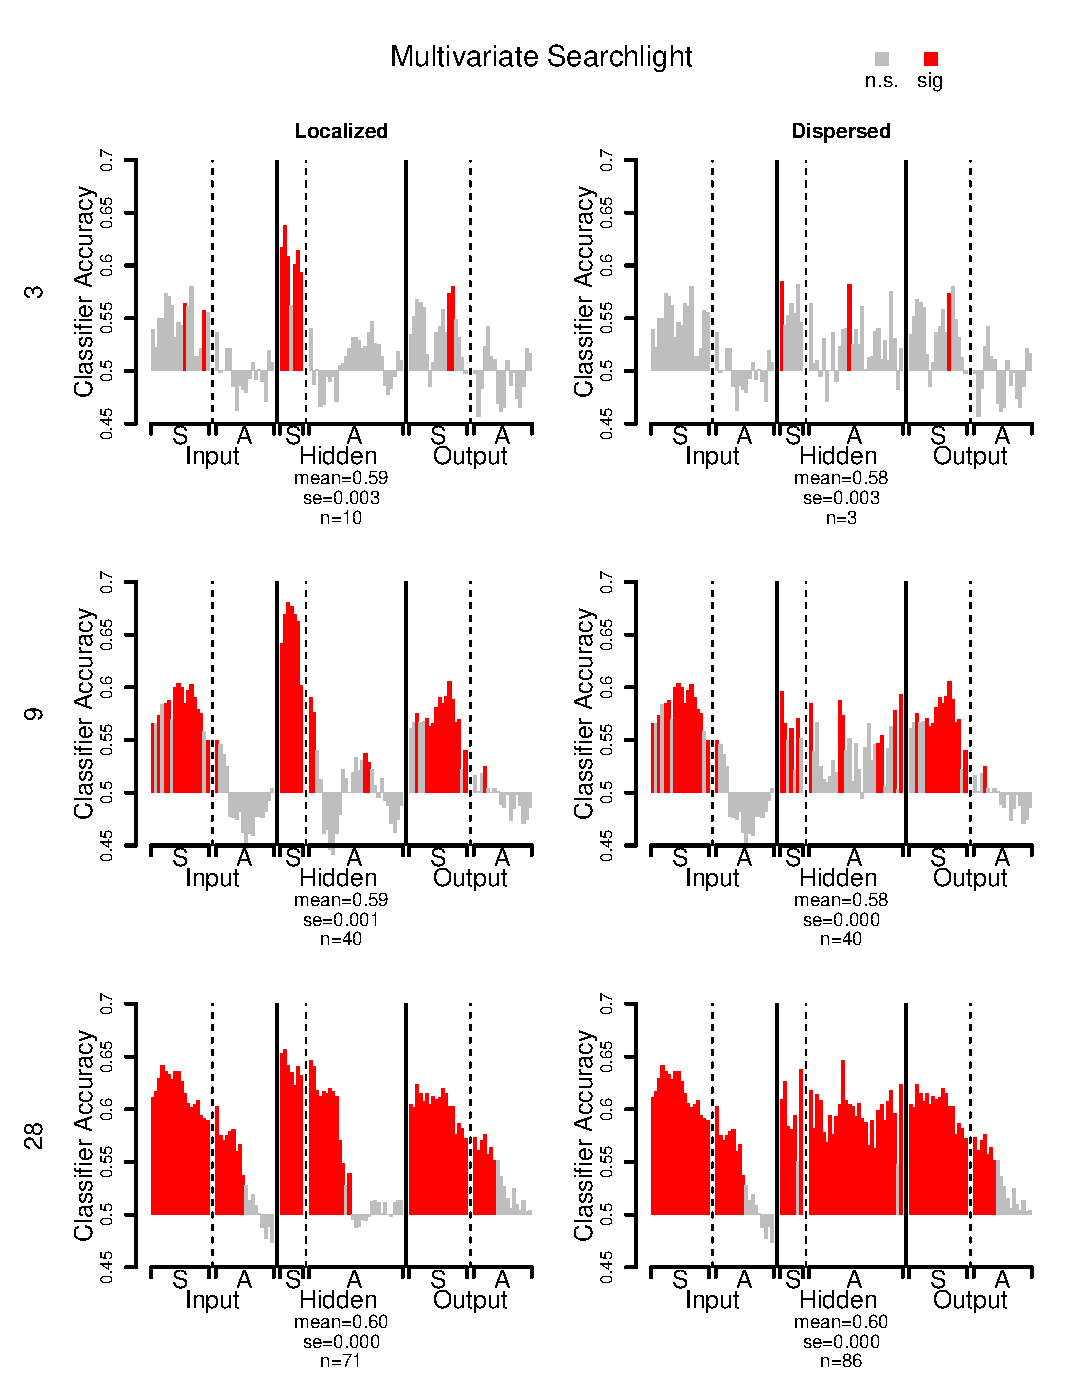
\includegraphics[width=0.85\textwidth]{figures/searchlight.eps}
\caption{\label{fig.searchlight} Result of the multivariate searchlight analysis of simulated data. Bar height indicates the mean classifier accuracy over subjects. Bars in red indicate searchlights where classification accuracy differed from chance over subjects, p-values corrected to control the false discovery rate at $q<0.05$. Results are presented for the searchlight sizes, indicated at the far left of each row.}
\end{figure}

Figure \ref{fig.searchlight} shows the results of the searchlight analyses, for localized and dispersed model architectures, and for different searchlight sizes. The format is the same as in the preceding analysis, except the y-axis now indicates the mean classification accuracy for spotlights centered on each unit, rather than a t-value at each unit. As before, colored bars indicate units that the method identifies as statistically significant---that is, units whose surrounding searchlights show classification accuracy reliably above chance across model individuals.

There are several points to note in these plots. First, when the hidden representations are anatomically localized, the method can do a quite good job of identifying both the systematic I/O and the systematic hidden units as important for the domain representations, though for both unit types the results vary substantially with the spotlight size. When the spotlight is small, the method reliably finds the SH units but misses most of the systematic I/O units. This happens because, as noted earlier, the SH units encode a clearer differentiation between domains, so that even if the spotlight does not encompass all 7 units there is sufficient information within it to classify stimuli above chance. The domain distinction is weaker in the systematic-I/O units, so when only a small number of such units fall within the spotlight, there is insufficient information to classify correctly. With a larger searchlight (9 units), the method does very well at finding all relevant units.  When it grows too large, however, it begins to incorrectly flag irrelevant units as being important for the representation (28 units). A very large spotlight, even when centered on an uninformative (arbitrary) unit, can have a broad enough span that it encompasses other informative units. In this case the classifier will perform well by virtue of the informative units appearing in the edge of the spotlight, but the above chance result will be ``stored'' in the spotlight center, making it appear as though there is useful information present at that location. Thus when the signal is anatomically localized, there is a tradeoff between spotlight size and discovery of representational structure, with spotlights that are too small missing weaker signal and those that are too large incorrectly flagging arbitrary signal.

In the model case, where we know {\it a priori} which are the signal-bearing units, it is easy to discern the optimal searchlight size, but it is less clear how this would be determined from real brain imaging data. One might initially expect the optimal searchlight to be identifiable from the accuracy of the resulting classifiers, but Figure \ref{fig.searchlight} suggests that this is not the case: the very large searchlight, which flags many irrelevant units, shows almost as good classifier performance as the optimal size at the SH units and better performance at the systematic I/O units. If we did not already know which units were important for representation in the model, it would be difficult to know which searchlight size to choose, and hence which results to believe.

The second thing to note is that the searchlight analysis does a much poorer job overall of identifying the SH units when these are anatomically dispersed (right panels of Figure \ref{fig.searchlight}). The poor performance arises because the precise anatomical location of the signal-carrying units is assumed to vary across individuals in this case. Within any individual model, a searchlight that includes a few of the informative units will show above-chance performance in classification, but the searchlight centers will differ across model individuals, especially when the searchlights are small. Thus the cross-subject statistical test at each location will yield a null result, leading to poor signal discovery. Larger searchlights will be more likely to contain the signal-carrying units, but also lead to poorer localization of the signal as already noted. 

In sum, the method deals with the over-fitting problem by only including a small number of contiguous voxels in each classifier---an approach which assumes that useful representational structure can be localized within the searchlight radius, in the same locations across subjects. When these assumptions are met, the approach does a good job of discovering representational structure, even if the representational code (i.e., the way that individual units respond to particular stimuli) is highly variable within and across individuals. The limitations noted above arise when the assumptions are violated---when representational structure is anatomically distributed across multiple spotlights (as when spotlights are too small in the localized case), or in different ways across individuals (as in the dispersed model). Moreover, whether the assumptions are met depends, not only upon the anatomical distribution of the signal, but also upon the searchlight size, and it is not clear how the latter can be optimized for real brain imaging data.  

Finally, it is worth noting that, in contrast to the univariate method, the searchlight approach does not provide information about how the contrast of interest in encoded in unit activations. Each searchlight returns a single number indicating how well its surround differentiates items from the two classes, but it does not indicate how the distinction is encoded in unit activations. Thus there is no way for the method to show, for instance, that there are some units systematically more active for A items than B items, others showing the reverse pattern, and still others that express the A/B distinction in a distributed code (the SH units).

Returning to the central questions, we get the following answers:

\begin{enumerate}
\item {\bf Does the method reliably identify the systematic I/O units?} Yes, though results vary substantially with searchlight size.
\item {\bf Does the method reliably identify the systematic hidden units?} Yes, when they are anatomically localized and when the searchlight is not too large.
\item {\bf Does the method indicate how the information of interest is coded across identified units?} No.
\item {\bf Do method results depend on anatomical localization of signal-carrying units?} Yes: performance declines substantially when signal-carrying units are anatomically dispersed.
\end{enumerate}
